Como mencionado anteriormente, este trabalho tem como objetivo construir e validar um código em linguagem de descrição de hardware para processar em tempo real as características de transferência de um amplificador, reproduzindo suas não linearidades e efeitos de memória. O projeto foi dividido em três etapas principais:

\begin{itemize}
\item Estudo do DPD;
\item Modelagem em software;
\item Implementação em FPGA;
\end{itemize}



\subsection{Estudo dos DPDs}
A etapa consistiu no estudo dos DPDs, onde foi feito todo o levantamento sobre os tipos de modelagem dos DPDs. O objetivo deste estudo é entender as diferentes abordagens de modelagem, avaliar seus desempenhos e identificar a mais adequada para a aplicação em amplificadores de potência.

\subsection{Implementação em software} \label{sec:implsoft}

Nesta etapa, foi realizada a implementação do modelo DPD em software, utilizando a linguagem de programação Python. Esta linguagem é amigável e amplamente difundida na comunidade acadêmica.

Para essa modelagem, foram coletados sinais de entrada e saída de um amplificador de potência classe AB, que utiliza um HEMT fabricado com tecnologia GaN. O amplificador foi excitado por um sinal portador de frequência de 900 MHz, modulado por um sinal de envelope WCDMA 3GPP com aproximadamente 3,84 MHz de largura de banda. Os dados de entrada e saída do amplificador de potência foram medidos usando um VSA Rohde \& Schwarz FSQ com uma taxa de amostragem de 61,44 MHz, conforme disponível em \cite{Bonfim2016}.

Em seguida, realizou-se o cálculo da estimativa do sinal utilizando números com vírgula fixa. Para verificar a precisão dessa estimativa em relação ao sinal original, calculou-se o NMSE. Para essa validação, os dados foram inicialmente divididos em conjuntos de extração e validação, que são dados utilizados para fazer o calculo do modelo e para fazer a validação do modelo calculado, respectivamente. A matriz de confusão foi calculada com os dados de extração. Esse cálculo é essencial para a extração dos coeficientes do polinômio de memória. Após a extração dos coeficientes, calculou-se o modelo do PA, que foi então validado com os dados de validação. O NMSE obtido para um polinômio de 2° grau com uma amostra memorizada foi de -23,57 dB.

Em seguida, o algoritmo foi ajustado para operar com números em vírgula fixa e o número total de bits foi reajustado para atingir a menor resolução possível, buscando o menor NMSE simulado. Por se tratar de um cálculo em virgula fixa, fez-se necessário uma readequação do resultado obtido entre cada multiplicação de forma a manter a resolução inicial.

\subsection{Implementação em FPGA}
Essa etapa consiste na implementação do DPD em FPGA. Para isso, é necessário realizar paralelizações nas operações aritméticas. A Figura \ref{fig:diagramaprocess} ilustra como esse processo está dividido entre cada ciclo de clock. A cada ciclo, duas operações são realizadas em paralelo: o sinal atual é elevado ao quadrado e registrado, enquanto ocorre o somatório do produto entre os sinais do mesmo instante de tempo e seus respectivos coeficientes. Esse processo ocorre P vezes para os \( P \) graus do polinômio de memória. Portanto, a saída do DPD é incompleta para os primeiros \( P \) períodos de clock, pois, nesses primeiros ciclos, realiza-se o cálculo com base em entradas de sinais anteriores que ainda não ocorreram, resultando em uma saída incompleta.

\begin{figure}[ht!]
  \centering
  \captionsetup{justification=centering}
  \caption*{Fonte: Autor}
  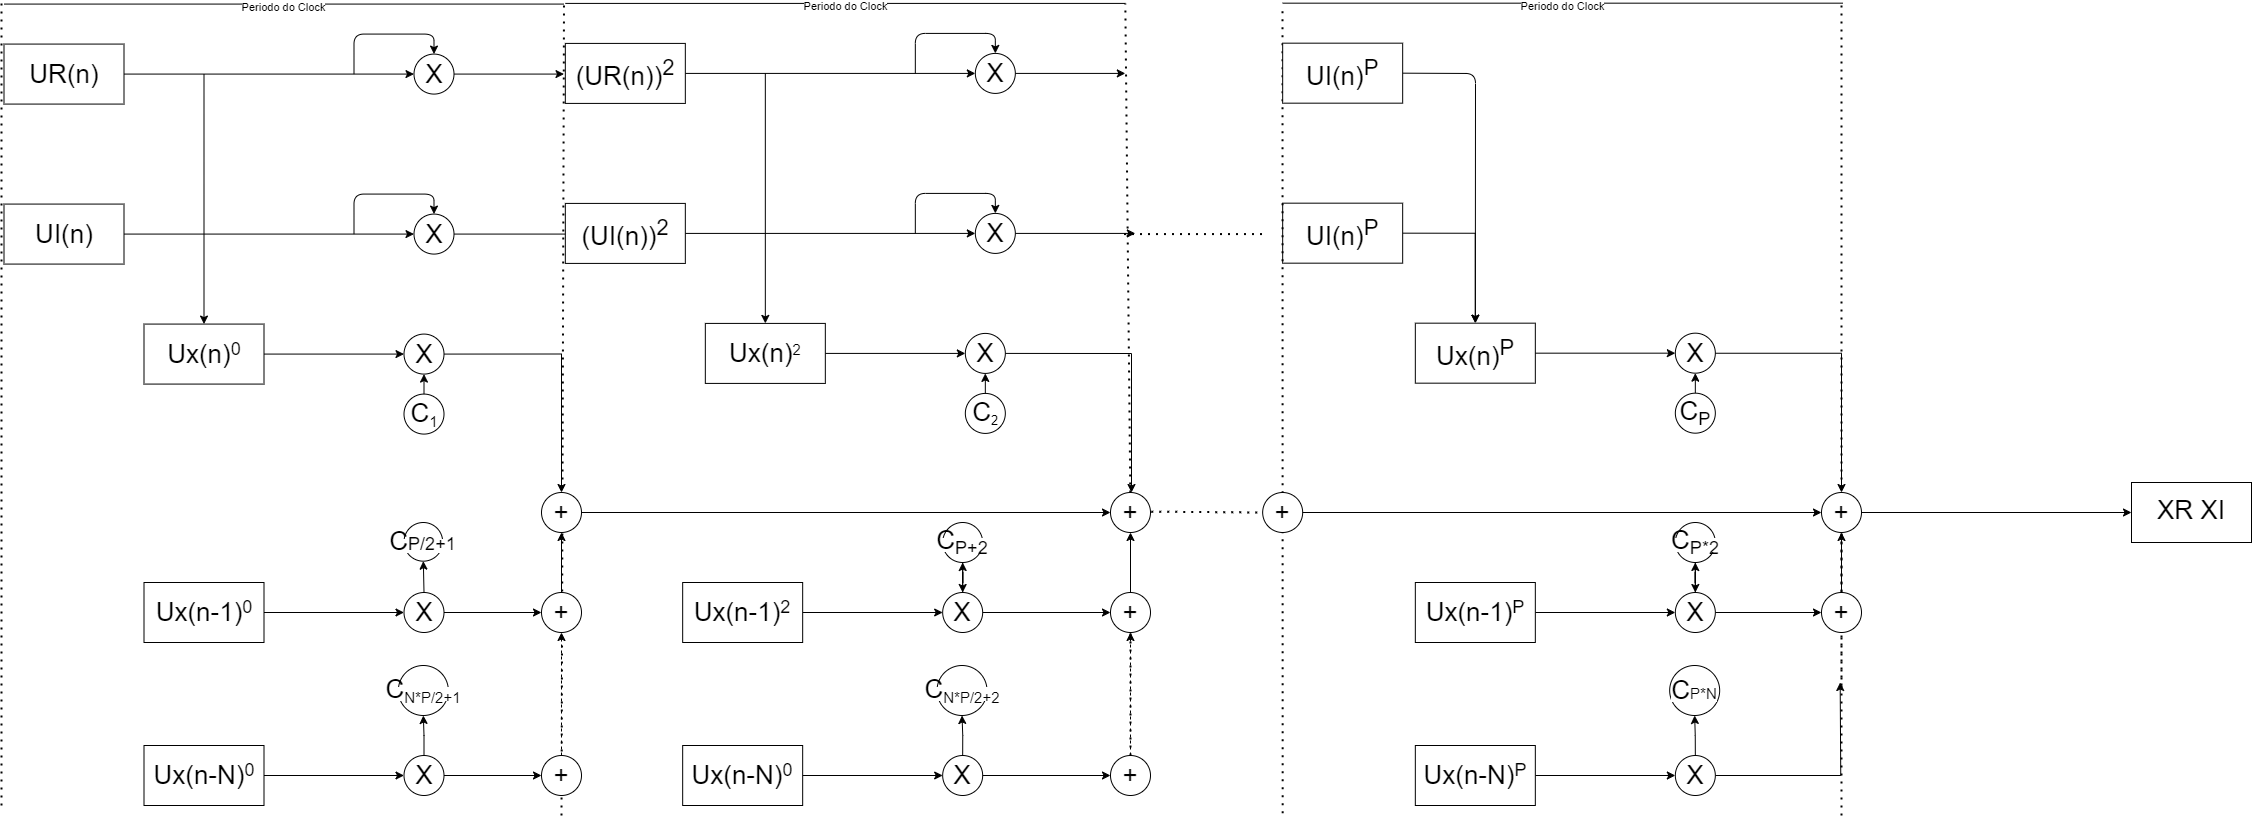
\includegraphics[width=1.0\textwidth]{diagrama_process.png}
  \caption{Processo de cálculo da saída}
  \label{fig:diagramaprocess}
\end{figure}
  
